\documentclass[12pt]{article}

\usepackage[spanish,activeacute]{babel}
\usepackage[utf8]{inputenc}
\usepackage{graphicx}
%\usepackage{fullpage}

\title{Ocultar datos en archivos de sonido}
\author{Juan Antonio Cano Salado \and Borja Moreno Fernández \and Pascual Javier Ruiz Benítez}

\begin{document}

\maketitle

\newpage
\tableofcontents

\newpage
\section{Resumen}

Este trabajo aborda la ocultación de datos en archivos de sonido o, lo que es lo mismo, la esteganografía de audio. El objetivo de esta disciplina consiste básicamente en ocultar información (de cualquier tipo) en archivos de sonido, de forma que los cambios llevados a cabo en el archivo original resulten imperceptibles para una persona.

Comenzaremos estudiando los principios básicos de la esteganografía en general, y de la esteganografía de audio en particular. A continuación, analizaremos algunos de los métodos más comúnmente utilizados en esteganografía de audio. Hecho esto, estudiaremos uno de los formatos de audio más populares: el formato WAV. Finalmente, incluiremos una descripción de la implementación realizada y proporcionaremos un manual de instalación y manejo de la aplicación desarrollada.

\section{Introducción}

\subsection{Esteganografía}

La esteganografía es la disciplina en la que se estudian y aplican técnicas que permiten el ocultamiento de mensajes u objetos, dentro de otros, llamados portadores, de modo que no se perciba su existencia.

Los orígenes de la esteganografía datan de la antigua Grecia. Heródoto, famoso historiador griego, informa del uso de la esteganografía en informes de Grecia a Persia. El método consistía en afeitar la cabeza de un esclavo y tatuar allí un mensaje. Dicho mensaje quedaba oculto cuando el pelo del esclavo volvía a crecer. Para leer el mensaje sólo era necesario volver a afeitarle la cabeza al esclavo. La idea era que nadie sospechase de la existencia de dicho mensaje.

La esteganografía ha sido usada en numerosas ocasiones a lo largo de la historia: tintas invisibles, acrósticos o mensajes microscópicos son sólo algunas de sus formas. Recientemente, en plena era digital, la estaganografía ha adquirido gran importancia como tecnología utilizada en el campo de la seguridad informática. Pueden ocultarse mensajes secretos en correos electrónicos, imágenes, audio e incluso vídeo.

Diversos grupos han mostrado tener un gran interés en las aplicaciones de la esteganografía. Algunos, interesados en la protección de derechos de autor. Otros, preocupados por proteger la privacidad de sus mensajes. Muchos gobiernos temen que la esteganografía podría convertirse en una herramienta de gran utilidad para criminales y grupos terroristas. En cualquier caso, parece claro que existen multitud de aplicaciones y usos para la esteganografía, y la mayoría de los expertos están de acuerdo en que será un tema de gran interés durante los próximos años.

La figura \ref{prisioneros} ilustra un ejemplo simple de un problema en el que el uso de la esteganografía puede ser de utilidad.

\begin{figure}[h]
  \centering
    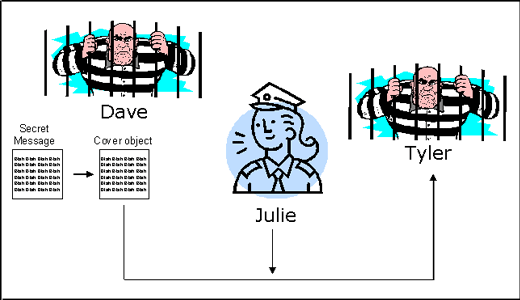
\includegraphics[width=\textwidth]{img/prisoners}
  \caption{Problema de los prisioneros}
  \label{prisioneros}
\end{figure}

Tyler y Dave están en la cárcel. Necesitan comunicarse para ultimar los detalles de un plan de fuga, pero tienen un gran problema: Julie, guardia de la prisión, tiene acceso a toda la correspondencia entre los prisioneros. La criptografía por sí sola no es una solución. Un mensaje cifrado levantaría todo tipo de sospechas. Los prisioneros deben idear un sistema que les permita pasar mensajes de apariencia inocente, con información oculta que sólo ellos puedan entender.

La esteganografía puede además combinarse con la criptografía para crear sistemas más seguros. Así, distinguimos:

\begin{itemize}

\item Esteganografía pura

La fortaleza del sistema recae en los algoritmos de ocultación y extracción de la información, que solo el emisor y el receptor del mensaje deberían conocer.

\item Esteganografía de clave privada

Fruto de la combinación de esteganografía pura con criptosistemas simétricos. Se asume que un atacante podría conocer los algoritmos de ocultación y extracción de la información. Por este motivo, el mensaje se cifra utilizando un cifrado simétrico antes de ocultarlo. De esta manera, incluso si el atacante intercepta la transmisión y logra extraer la información aún tendrá que enfrentarse al criptoanálisis del criptosistema utilizado.

\item Esteganografía de clave pública

Basada en unir esteganografía pura y criptosistemas de clave pública. De esta manera, el emisor y el receptor evitan tener que compartir una clave privada.

\end{itemize}

\subsection{Audio digital}

El audio digital se diferencia del sonido analógico tradicional en que es una señal discreta en lugar de una señal continua. Esta señal discreta es creada llevando a cabo un proceso de muestreo y cuantización de una señal analógica continua. La frecuencia de muestro varía según los propósitos. Por ejemplo, la frecuencia de muestreo estándar para un CD de audio digital es de alrededor de 44kHz. La figura \ref{audiodigital} ilustra el proceso de muestro y cuantización para producir una señal de audio digital a partir de una señal continua de audio analógico.
En dicha figura se ha exagerado la naturaleza discreta de la señal digital. Sin embargo, las frecuencias de muestreo usuales permiten que el audio digital sea prácticamente idéntico a la señal de audio analógica original.

\begin{figure}[h]
  \centering
    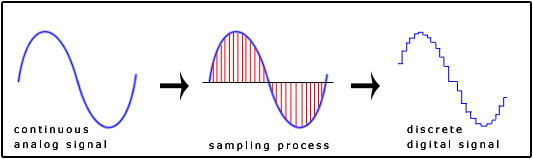
\includegraphics[width=\textwidth]{img/digitalaudio}
  \caption{Audio digital}
  \label{audiodigital}
\end{figure}

Los archivos de audio digital se almacenan en el ordenador como una secuencia de ceros y unos. Con las herramientas apropiadas, es posible alterar individualmente los bits que componen estos archivos. Esto hará posible llevar a cabo modificaciones a la secuencia binaria que produzcan cambios en la señal de audio que no sean perceptibles al oído humano.

\subsection{Esteganografía de audio}

En un sistema de estaganografía digital informatizado, se ocultan mensajes secretos en audio digital. El mensaje secreto se introduce alterando ligeramente la secuencia binaria del archivo de audio. Existen aplicaciones de esteganografía de audio que permiten ocultar mensajes en archivos de audio en formato WAV, AU e incluso MP3.

Ocultar mensajes secretos en archivos de sonido suele ser más difícil que ocultar mensajes en archivos de imagen o vídeo. Esto se debe a la mayor sensibilidad que presenta en las personas el sistema auditivo frente al sistema visual. Existen un buen número de métodos y algoritmos para llevar a la práctica estos conceptos, algunos de ellos sencillos y otros más complejos (basados en técnicas avanzadas de procesado digital de señales). Estos métodos serán analizados en mayor detalle en la sección ``Soluciones presentadas".

\newpage
\section{Descripción del problema}

\newpage
\section{Soluciones presentadas}

\newpage
\section{Conclusiones}

\newpage
\section{Problemas abiertos}

\newpage
\section{Implementación realizada}

\newpage
\section{Manual de instalación y manejo de la aplicación}

\newpage
\section{Bibliografía}

\newpage
\section{Tabla de tiempo}

\end{document}